\pdfminorversion=3
\documentclass[tikz]{standalone}
\usepackage{vuiprepstandalone}
\usepackage{alain2}
\usepackage[locale=FR]{siunitx}



\begin{document}
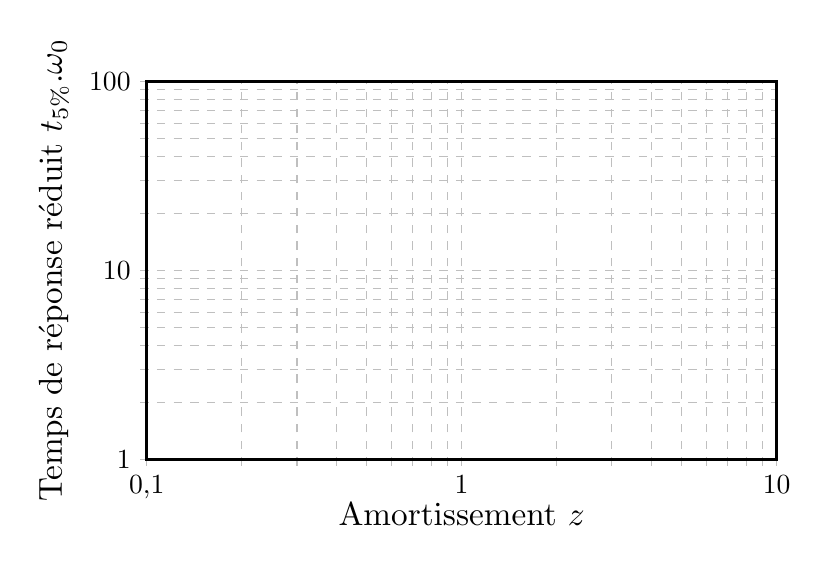
\begin{tikzpicture}[scale=0.8]
\foreach \x in {0.1,0.2,0.3,0.4,0.5,0.6,0.7,0.8,0.9,1,2,3,4,5,6,7,8,9,10} {
\draw[dashed,gray!50] ({log10(\x)*5},-0.1) -- ({log10(\x)*5},6);
}
\foreach \x in {1,2,3,4,5,6,7,8,9,10,20,30,40,50,60,70,80,90,100} {
\draw[dashed,gray!50] (-5.1,{log10(\x)*3}) -- (5,{log10(\x)*3});
}
\node[below] at (-5,-.1) {\numprint{0,1}};
\node[below] at (0,-.1) {\numprint{1}};
\node[below] at (5,-.1) {\numprint{10}};
\node[left] at (-5.1,0) {\numprint{1}};
\node[left] at (-5.1,3) {\numprint{10}};
\node[left] at (-5.1,6) {\numprint{100}};
\node[below,scale=1.2] at (0,-.5) {Amortissement $z$};
\node[below,rotate=90,scale=1.2] at (-6.9,3) {Temps de réponse réduit $t_{5\%}.\omega_0$};
\draw[xscale=5,yscale=3,very thick,cyan] plot file {02PerformancesSLCI/ex_Telechirurgie2/images/abaque_tr5_0.1_10_log.table};
\draw[very thick] (-5,0) rectangle (5,6);
\end{tikzpicture}
\end{document}
